\chapter{Framework and Strategies Evaluation}
\label{chap:strategies}

This chapter visualizes the data collected from the test runs with the various
proposed strategies. The first part of the chapter explains the data obtained
and compares them to the expected results for each strategy described in
\sect{sec:strategies}. The second part of the chapter shows the scores of the
strategies when the obtained data are fitted to the model discussed in
\ssec{ssec:model}. The latter part of the chapter discusses suggested
improvements to the model for a better strategiey juxtaposition.

\section{Tests}
Tests that cover all the combinations between sending strategies and receivers
strategies have been run.  All of them have the same terminating condition that
is reached when at least one node finds a safety oracle at height 4 (in other
words, that the block at height 4 in a node's view is finalized). The number of
nodes is chosen at random in the interval \([2, 20[\). Performing tests on this
interval is large enough to give an insight on the interactions between all the
metrics and small enough to reach the terminating condition in a reasonable
amount of time (1 run with a number of nodes chosen at random takes on average 1
hour with the Maximal overhead strategy). Because the Maximal overhead strategy
takes way more time than the others to give results, this strategy has first
been run with a number of nodes in the interval \([2,10[\), then with the whole
\([2, 20[\) a lower number of times to confirm the tendencies observed with the
lower number of nodes.

\section{Visualization All receivers}
This section presents a visualization of the data obtained through the multiple
test runs with the All receivers strategy.  Each subsection shows the results
using 3 histograms, representing the raw data, followed by 3 scatter plots
picturing each metric against one another. These graphs also show a simple linear
regression as an attempt to find a relation between each metric. At the end of
the chapter a linear regression is performed in order to
find the scores of each variable according to the model presented in
\ssec{ssec:model}.

\subsection{Round-robin}
\FloatBarrier
The distributions of the number of nodes and the latency
(\fig{fig:distRR} top row) have the same
shapes except for the gaps every 3 steps. The resemblance in shape is explained
by the fact that the latency is strictly correlated to the number of nodes, as
expected.
The gaps will be explained at the end of the section, using the graphs that show
relations between variables.

\triplefigure
    {hist_nb_nodes_rr_20_nodes_4_depth_all_receivers_gen_averages}
    {hist_latency_rr_20_nodes_4_depth_all_receivers_gen_averages}
    {hist_overhead_rr_20_nodes_4_depth_all_receivers_gen_averages}
    {Distributions of the dataset for the round-robin strategy and all
    receivers. As the latency (top-right) presents a linear correlation with the number of
    nodes (top-left), the shapes of the histograms are similar. The overhead
    (bottom) always equals to $\protect 1$ because only one message is sent per step, and each step
    finalizes a block.}
    {fig:distRR}

The histogram for the overhead is easy to analyse as well; the overhead is
expected to be $1$ because once consensus is obtained for the genesis block, only
one message from the next validator is needed to finalize the next block.

\triplefigure
    {relation_nb_nodes_latency_rr_20_nodes_4_depth_all_receivers_gen_averages}
    {relation_nb_nodes_overhead_rr_20_nodes_4_depth_all_receivers_gen_averages}
    {relation_overhead_latency_rr_20_nodes_4_depth_all_receivers_gen_averages}
    {The round-robin strategy shows a linear relation between the number of
    nodes and the latency (top-left). The overhead is a constant for this
    strategy (top-right, bottom).}
    {fig:relRR}

The right and center graphs on \fig{fig:relRR} do not give more insight on the
data, as the Overhead is always \(1\). On the other hand, the graph on the left
shows a clear linear relationship between the latency and the number of nodes.
The fitted line has the following equation:
\[l = 1.403402\cdot n\]
The latency is expected to be around \(1.5\cdot n\) because the finality is
reached when at least 50\% of the network has acknowledged that the whole
network has the finalized message in its justification. As pictured in the
top-left graph of \fig{fig:relRR}, the fitted line has a slightly small
slope compared to the data points due to the fact that the line is fitted to be
linear and the data points are close the origin. 
The gaps in the histogram for latecy showed in \fig{fig:distRR} are explained by the fact
that we expect the relation to be \(l = 1.5\cdot n\), and therefore the span of
the latency distribution is bigger than the one for the number of nodes. The
regularity of the gaps (which appear to be every 3 units of latency), is caused
by the regularity of the sending and receiving strategies. As all nodes receive
the messages at the same time they all finalize the same blocks together and
there cannot be a non-integer average value for the latency in this case.

\FloatBarrier
\subsection{Double round-robin}
\label{ssec:doubleRR}
\triplefigure
    {hist_nb_nodes_double_rr_20_nodes_4_depth_all_receivers_gen_averages}
    {hist_latency_double_rr_20_nodes_4_depth_all_receivers_gen_averages}
    {hist_overhead_double_rr_20_nodes_4_depth_all_receivers_gen_averages}
    {Distributions of the dataset for the double round-robin strategy and all
    receivers. As the latency (top-right) and the number of nodes (top-left) are
    linearly correlated, their distributions are of similar shapes. The
    overhead (bottom) equals 2, as expected and shows an outlying value at 4.}
    {fig:distDRR}

As for the simple round-robin case, the latency and number of nodes
distributions show a similar shape. The latency is more localized than for the
single round-robin and demonstrates a difference between distributions. The
distribution of the overhead presents a peak at 2, which was expected, but also
shows that there are some messages that have double this overhead at 4. The
appearence of these outliers is explained further in \ssec{ssec:arbitrary}. 

\triplefigure
    {relation_nb_nodes_latency_double_rr_20_nodes_4_depth_all_receivers_gen_averages}
    {relation_nb_nodes_overhead_double_rr_20_nodes_4_depth_all_receivers_gen_averages}
    {relation_overhead_latency_double_rr_20_nodes_4_depth_all_receivers_gen_averages}
    {The double round-robin strategy shows a linear relation between the number of
    nodes and the latency (top-left). The overhead is a constant for this
    strategy (top-right, bottom). The top-right plot indicates that the outliers
    only emerge when the tests are run with 3 or 5 nodes.}
    {fig:relDRR}

As for the simple round-robin strategy, the plots including the Overhead are not
of much use here, except they show that its value is 2, as it is expected. 
On the other hand, the plot on the top-left of \fig{fig:relDRR} shows a
linear relation between the number of nodes and the latency: 
\[l = 0.721750 \cdot n\]

The coefficient of this latency in relation to the number of nodes is about half
that of one signe round-robin method. The double round-robin strategy was
supposed to show half the latency with respect to the simple round-robin and
this value is therefore correct. The value of 2 for the overhead is also twice
the overhead for the single round-robin and confirms the hypothesis.
    

\FloatBarrier
\subsection{Triple round-robin}
\label{ssec:tripleRR}
The triple round-robin strategy shows  the same kind of information as the
double round-robin one. The overhead is 3 for almost all cases (this will be
discussed later), and the number of nodes and latency are linearly correlated.
\triplefigure
    {hist_nb_nodes_triple_rr_20_nodes_4_depth_all_receivers_gen_averages}
    {hist_latency_triple_rr_20_nodes_4_depth_all_receivers_gen_averages}
    {hist_overhead_triple_rr_20_nodes_4_depth_all_receivers_gen_averages}
    {Distributions of the dataset for the triple round-robin strategy and all
    receivers. As the latency (top-right) and the number of nodes (top-left) are
    linearly correlated, their distributions are of similar shapes. The
    overhead (bottom) equals 3, as expected and shows two outlying values at 1
    and 6.}
    {fig:distTRR}

The relationship with the overhead are again not of much use because its value
is always 3. Again, there is a linear relationship between the latency and the
number of nodes, which follows this equation:
    \[l = 0.496152 \cdot n\]
This coefficient is about a third that of the single round-robin method and the
overhead is three times larger.
\fig{fig:relTRR} shows clear outliersfor the overhead value when running
2, 5 and 11 nodes. When running 2 nodes, which is an obvious edge case for this
strategy (as there are only 2 nodes and there should be at least 3 to send
different messages), the overhead is only 1 because only one node sends a
message in this case. The appearence of the other two outliers is explained further in
\ssec{ssec:arbitrary}. 

\triplefigure
    {relation_nb_nodes_latency_triple_rr_20_nodes_4_depth_all_receivers_gen_averages}
    {relation_nb_nodes_overhead_triple_rr_20_nodes_4_depth_all_receivers_gen_averages}
    {relation_overhead_latency_triple_rr_20_nodes_4_depth_all_receivers_gen_averages}
    {The triple round-robin strategy shows a linear relation between the number of
    nodes and the latency (top-left). The overhead is a constant for this
    strategy (top-right, bottom) except for some outliers. The top-right plot
    indicates that the overhead is lower for 2 nodes, which is expected because
    fewer than 3 messages are sent in this case. Outliers are also found when
    running 5 and 11 nodes.}
    {fig:relTRR}

\FloatBarrier
\subsection{Maximal overhead}
This strategy aims to reduce latency to its minimum, as shown in the
top-right plot on \fig{fig:distOverhead}. The distributions of the number
of nodes and overhead are of the same shape because they are lineraly
correlated, as will be shown in the next paragraph. 
Note that the experiments were run with a lower number of nodes because the
simulations for a large number of nodes takes a large amount of time. The
simulations are currently implemented following the mathematical formulae found
in \cite{abstractCBC} and not yet optimized. For the sake of completion, a few runs
have been performed with the same amount of nodes as for the other experiments
to show whether or not there were divergences. It turned out that there was not
such divergences. 

\triplefigure
    {hist_nb_nodes_overhead_10-20_nodes_4_depth_all_receivers_gen_averages}
    {hist_latency_overhead_10-20_nodes_4_depth_all_receivers_gen_averages}
    {hist_overhead_overhead_10-20_nodes_4_depth_all_receivers_gen_averages}
    {Distributions of the dataset for the maximal overhead strategy and all
    receivers. As the overhead (bottom) and the number of nodes (top-left) are
    linearly correlated, their distributions are of similar shapes. The
    latency (top-righ) equals 2, as expected. Note that because the maximal
    overhead strategy is computationally heavy, tests were run for 10 nodes and
    a few of them were run for 19 nodes, which is reflected in the shapes of the
    bottom and top-left histograms.}
    {fig:distOverhead}

The top-right plot on \fig{fig:relOverhead} shows a linear dependency between
overhead and number of nodes of \(o = n\), as was expected.  The two other plots
on the same Figure only confirm that the latency equals 2, which is the minimum
that can be reached, as there needs to be two steps to finalize a message.
During the first step, all nodes acknowledge they have seen a message, and the
second step confirms that everyone has seen the other nodes acknowledgments.

\triplefigure
    {relation_nb_nodes_latency_overhead_10-20_nodes_4_depth_all_receivers_gen_averages}
    {relation_nb_nodes_overhead_overhead_10-20_nodes_4_depth_all_receivers_gen_averages}
    {relation_overhead_latency_overhead_10-20_nodes_4_depth_all_receivers_gen_averages}
    {The maximal overhead  strategy shows a linear relation between the number of
    nodes and the overhead (top-right). The latency is a constant for this
    strategy (top-left, bottom).}
    {fig:relOverhead}

\FloatBarrier
\subsection{Arbitrary}
\label{ssec:arbitrary}
This strategy is the only one that uses a random factor and that can be
considered as a "bottom-up" strategy. The main goal of this strategy is to
have a reference point when comparing new strategies.
The overhead distribution \todo{what is this shape? how to compute
characteristics?}

\triplefigure
    {hist_nb_nodes_arbitrary_20_nodes_4_depth_all_receivers_gen_averages}
    {hist_latency_arbitrary_20_nodes_4_depth_all_receivers_gen_averages}
    {hist_overhead_arbitrary_20_nodes_4_depth_all_receivers_gen_averages}
    {Distributions of the dataset for the arbitrary strategy and all
    receivers. Only the overhead seems to be distributed in a \todo{name of
    distrib} manner. }
    {fig:distArbitrary}

The top-left graph on \fig{fig:relArbitrary} shows a linear relationship
between the latency and the number of nodes. The equation of the fitted line is:
\[l = 2.091255 \cdot n\]
Though the slope varies a bit, it is still very similar to that of the simple
round-robin strategy.

The two other graphs on the Figure are less straightforward to explain than the
previous strategies'. The plot that pictures the relationship between the
overhead and the number of nodes shows two linear branches that split quite
clearly, and the same goes for the plot of the latency against the overhead.
The latter one shows an even weirder artifact: 

\triplefigure
    {relation_nb_nodes_latency_arbitrary_20_nodes_4_depth_all_receivers_gen_averages}
    {relation_nb_nodes_overhead_arbitrary_20_nodes_4_depth_all_receivers_gen_averages}
    {relation_overhead_latency_arbitrary_20_nodes_4_depth_all_receivers_gen_averages}
    {The arbitrary strategy shows a linear relation between the number of
    nodes and the latency (top-left). However, the other relations between
    variables both seem to be split into two linear functions with a clear gaps
    between them.}
    {fig:relArbitrary}

During the analysis phase of this strategy and particularly when trying to
explain the straight line appearing on the bottom-left graph on
\fig{fig:relArbitrary}, a critical bug was discovered. This bug happens when two
or more messages are finalized during the last step of the simulation. As the
bug was identified near the end of the projet's tomeframe, it was not corrected,
but will require to be fixed in order to continue research on the subject. As
the data collection process is segregated from the metrics computations
(\ssec{ssec:metricsMeasurements}), data that has elready been generated are not
lost and can be used again when the bug is corrected. Note that this bug also
explains the outliers observed for the Double round-robin and Triple round-robin
strategies as well (\ssec{ssec:doubleRR} and \ssec{ssec:tripleRR}).
Nonetheless, a version of the graphs with the edge cases filtered out was made
in order to better benchmark the strategy (\fig{fig:relArbitraryFiltered}).

\triplefigure
    {relation_nb_nodes_latency_arbitrary_filtered_20_nodes_4_depth_all_receivers_gen_averages}
    {relation_nb_nodes_overhead_arbitrary_filtered_20_nodes_4_depth_all_receivers_gen_averages}
    {relation_overhead_latency_arbitrary_filtered_20_nodes_4_depth_all_receivers_gen_averages}
    {The arbitrary strategy shows a linear relation between the number of
    nodes and the latency (top-left). However, the other relations between
    variables both seem to be split into two linear functions with a clear gaps
    between them.}
    {fig:relArbitraryFiltered}


\todo{finish analysis}

\FloatBarrier
\subsection{Fitting of the basic model}
\label{ssec:fittingBase}
Fitting the basic model described in \ssec{ssec:model} (\(1 = s_n \cdot
\frac{1}{n} + s_l\cdot l + s_o\cdot o\)) to the data using a simple linear
regression gives the results as shown as raw values on \tab{fig:recapTests} and
in a bar graph on \fig{fig:recapTestsPlot}.

\begin{table}[h]
    \centering{
        \begin{tabular}{|c|c|c|c|c|}
            \hline
            Sending Strategy & \(s_n\) & \(s_l\) & \(s_o\) & RMSE \\
            \hline
            Round-robin        & 0.000 & 0.000 & 1.000 & 0.000\\
            \hline
            Double round-robin & 1.435 & 0.055 & 0.162 & 0.141\\
            \hline
            Triple round-robin & 1.686 & 0.084 & 0.091 & 0.115\\
            \hline
            Maximal overhead   & 0.000 & 0.500 & 0.000 & 0.000\\
            \hline
            \hline
            Arbitrary          & 2.556 & 0.026 & 0.002 & 0.233\\
            \hline
        \end{tabular}
        %\captionsetup{justification=centering}
        \caption{Raw fitted values for the simple model, rounded to the 3rd
        decimal place. The RMSE column shows the error value for the linear
        regression. The rows for both round-robin and maximal overhead are both
        expected; the round robin strategy maximizes the overhead score and the
        maximal overhead strategy maximizes the latency score. The score for the
        latency increases with the number of message per step as the score for
        the overhead decreases. The score for the number of nodes seems to be a
        buffer that depends on how bad the two other scores are, which is
        confirmed by the error that increases with it.}
        \label{fig:recapTests}
    }
\end{table}

The scores obtained for the round-robin and the maximal overhead strategies are
the expected ones. The round-robin strategy optimizes the overhead (one message
per new finalized block) and the latency evolves linearly with the number of
nodes and is therefore bad. The score for the number of nodes will be discussed
later in this chapter. The maximal overhead strategy shows that it maximizes the
latency (which is \(2\), the minimal value for the latency) and therefore the
rest of the scores are non influential.
For the double and triple round-robin strategies, the variation for the overhead
and the latency scores, compared to the ones for the round-robin are also in
accordance with what is expected; the latency decreases when the number of
rounds augments and the overhead increases along with the number of nodes
sending messages in a single round.

\begin{figure}[h]
    \centering
    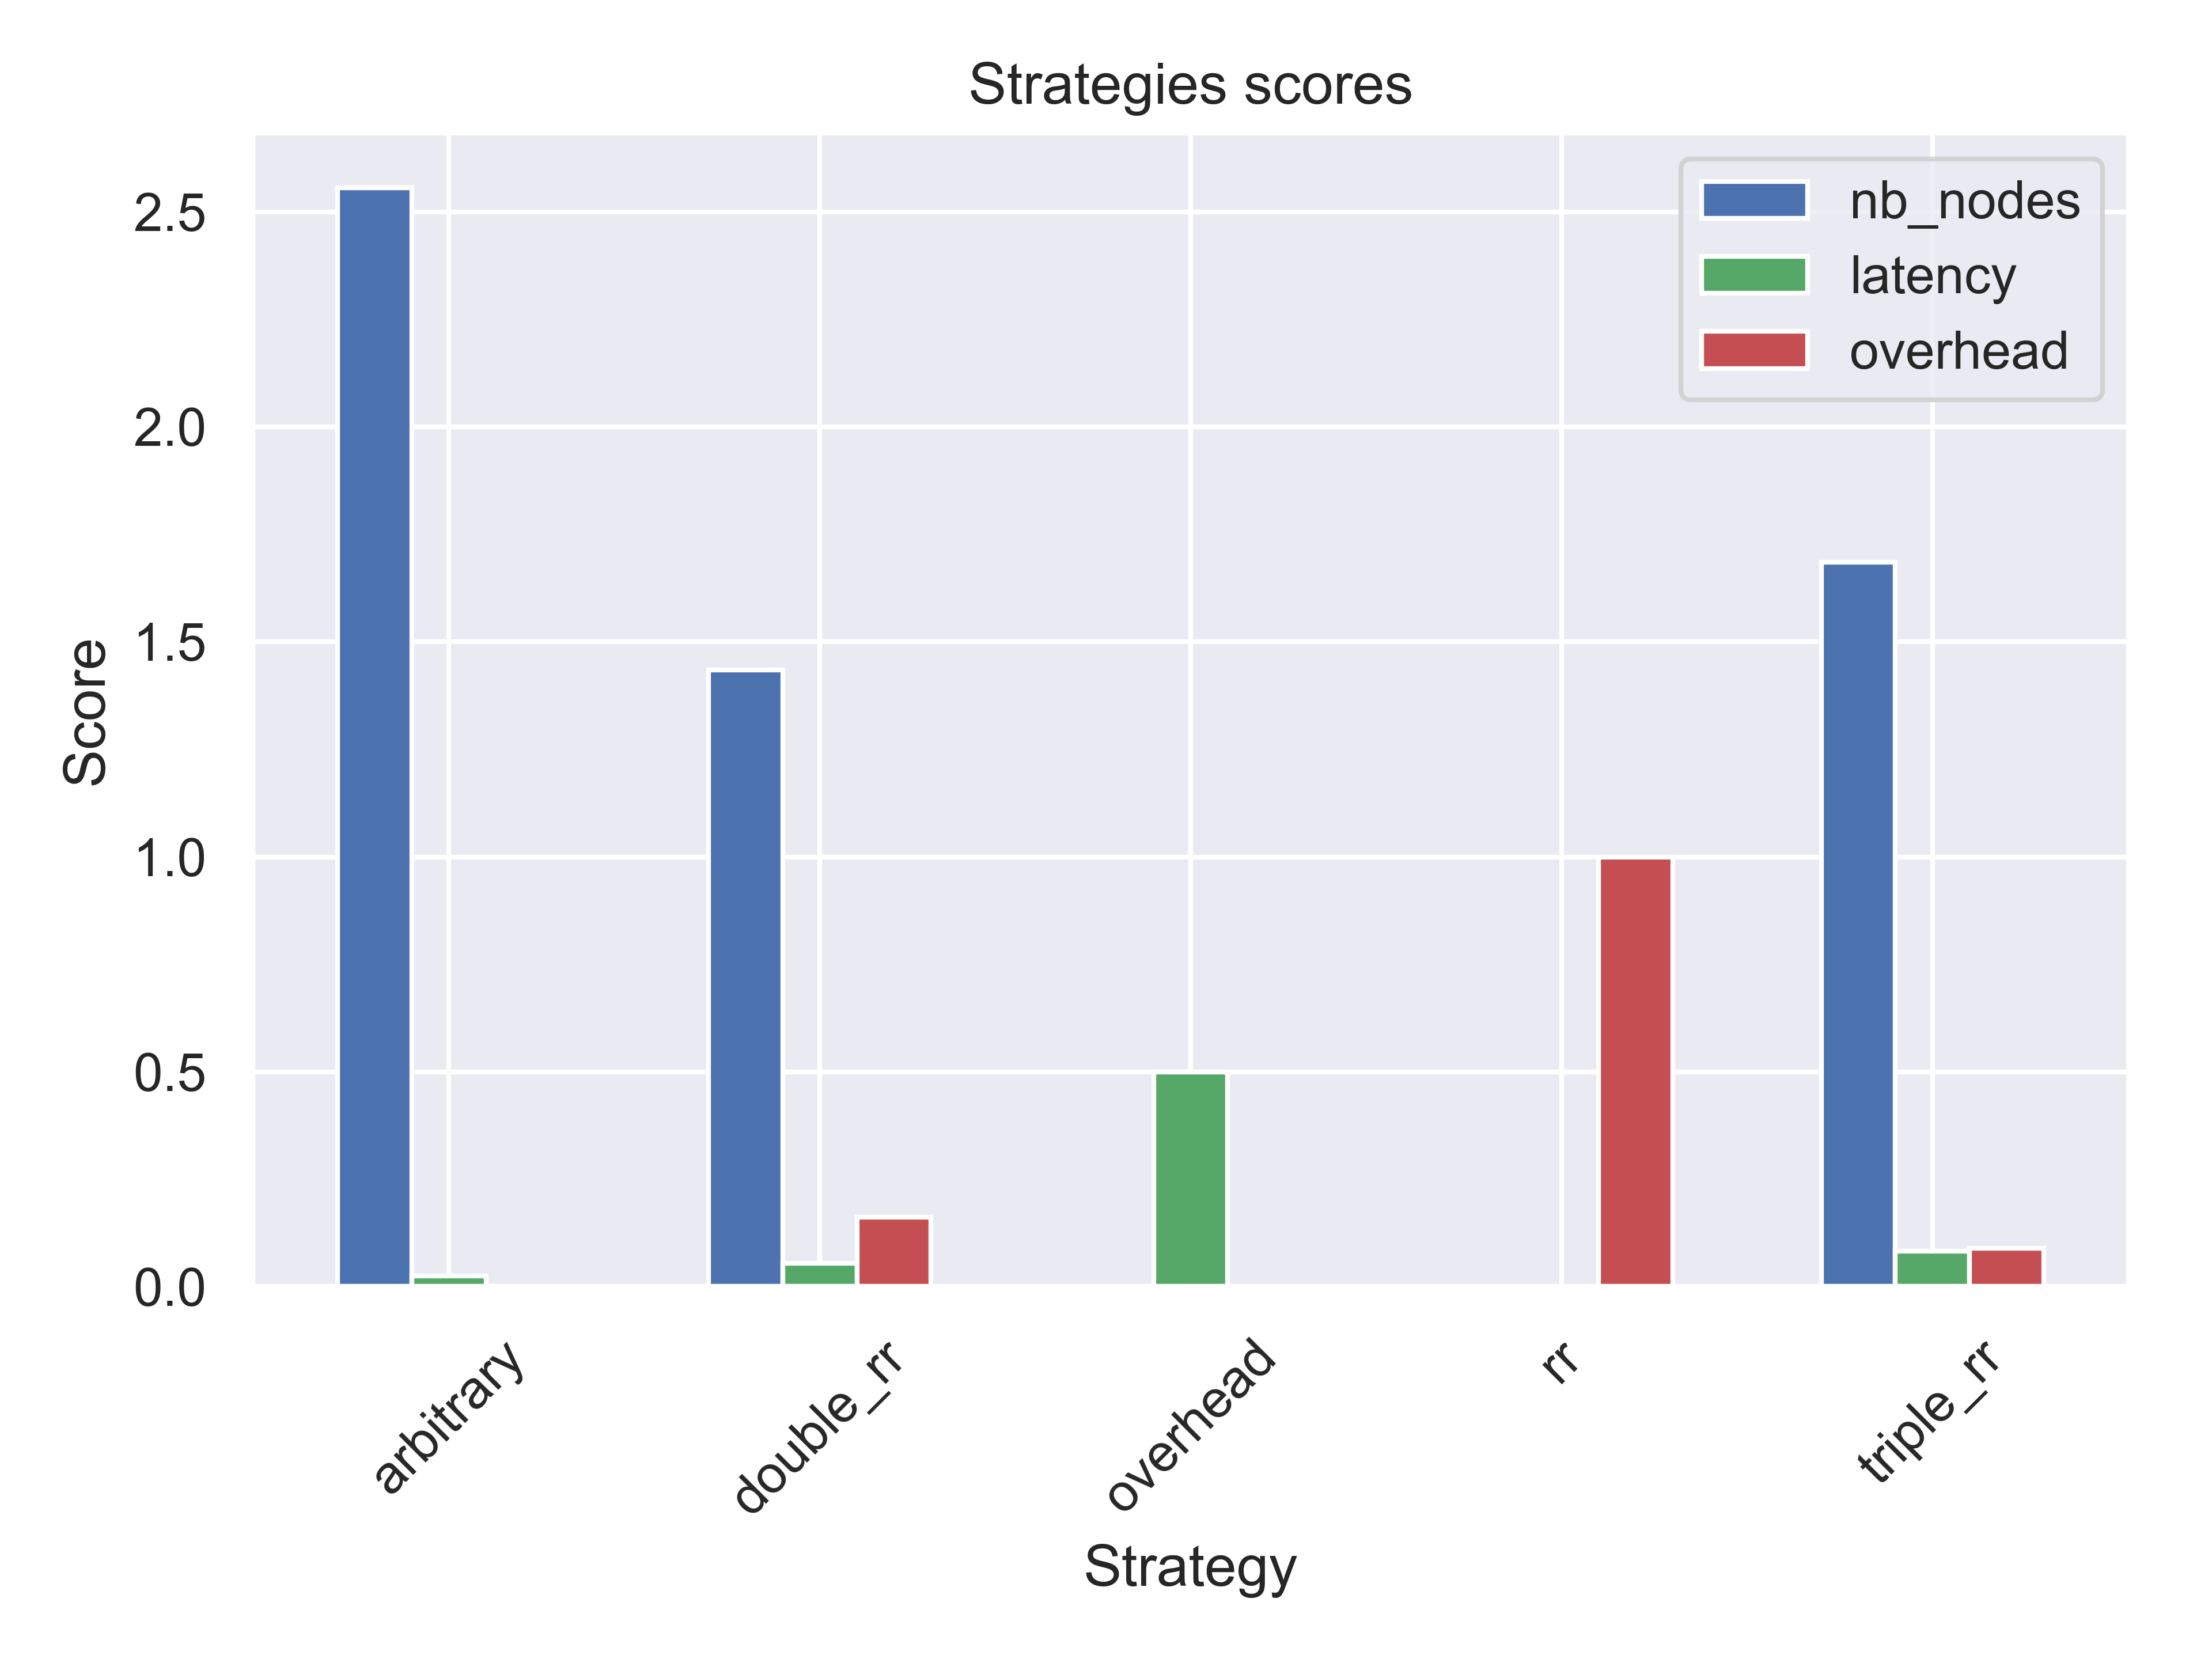
\includegraphics[width=0.8\columnwidth]{final_plot_basic_model}
    %\captionsetup{justification=centering}
    \caption{Raw fitted values for the simple model. The strategies are listed
    on the x-axis and their scores are plotted along the y-axis. The RMSE column shows the error value for the linear
        regression. The rows for both round-robin and maximal overhead are both
        expected; the round robin strategy maximizes the overhead score and the
        maximal overhead strategy maximizes the latency score. The score for the
        latency increases with the number of message per step as the score for
        the overhead decreases. The score for the number of nodes seems to be a
        buffer that depends on how bad the two other scores are, which is
        confirmed by the error that increases with it.
    }
    \label{fig:recapTestsPlot}
\end{figure}

\subsubsection{Number of nodes}
\label{ssec:nbNodes}
The main problem with these results is the evolution of the score for the number
of nodes, particularly for the arbitrary strategy. Based on the observations
made in \ssec{ssec:arbitrary}, the arbitrary strategy is clearly worse than the
others ones for the latency and overhead which is reflected with the values
obtained for their respective scores. The main issue with the arbitrary strategy
relies in the fact that \(s_n\) serves as a buffer for how well the other two
variables perfom in a given strategy.  Indeed, the model forces the relation
between the scores and the variables, and if the scores for both the latency and
the overhead are low, the score for the number of nodes is forced to be high.
Furthermore, the number of nodes is the variable with the lowest variance so the
fitting shows a lower error by using it as a buffer instead of the two others.
This is confirmed by looking at the error column in \tab{fig:recapTests}; the
bigger the score for number of nodes is, the higher the error. 

\FloatBarrier
\subsection{Normalized model}
\fig{fig:recapTestsPlotNorm} presents a normalized visualization of the same
data in \fig{fig:recapTestsPlot}. The normalization is made per-class, i. e.
each class is normalized against the best score for that class. This
normalization mainly permits to better visually compare the strategies on a
per-class basis. It also shows a correlation between the scores for the number
of nodes and the error values, which further confirms that the score for the
number of nodes is used as a buffer when the two other scores are sub-par and
don't fit the model.


\begin{figure}[h]
    \centering
    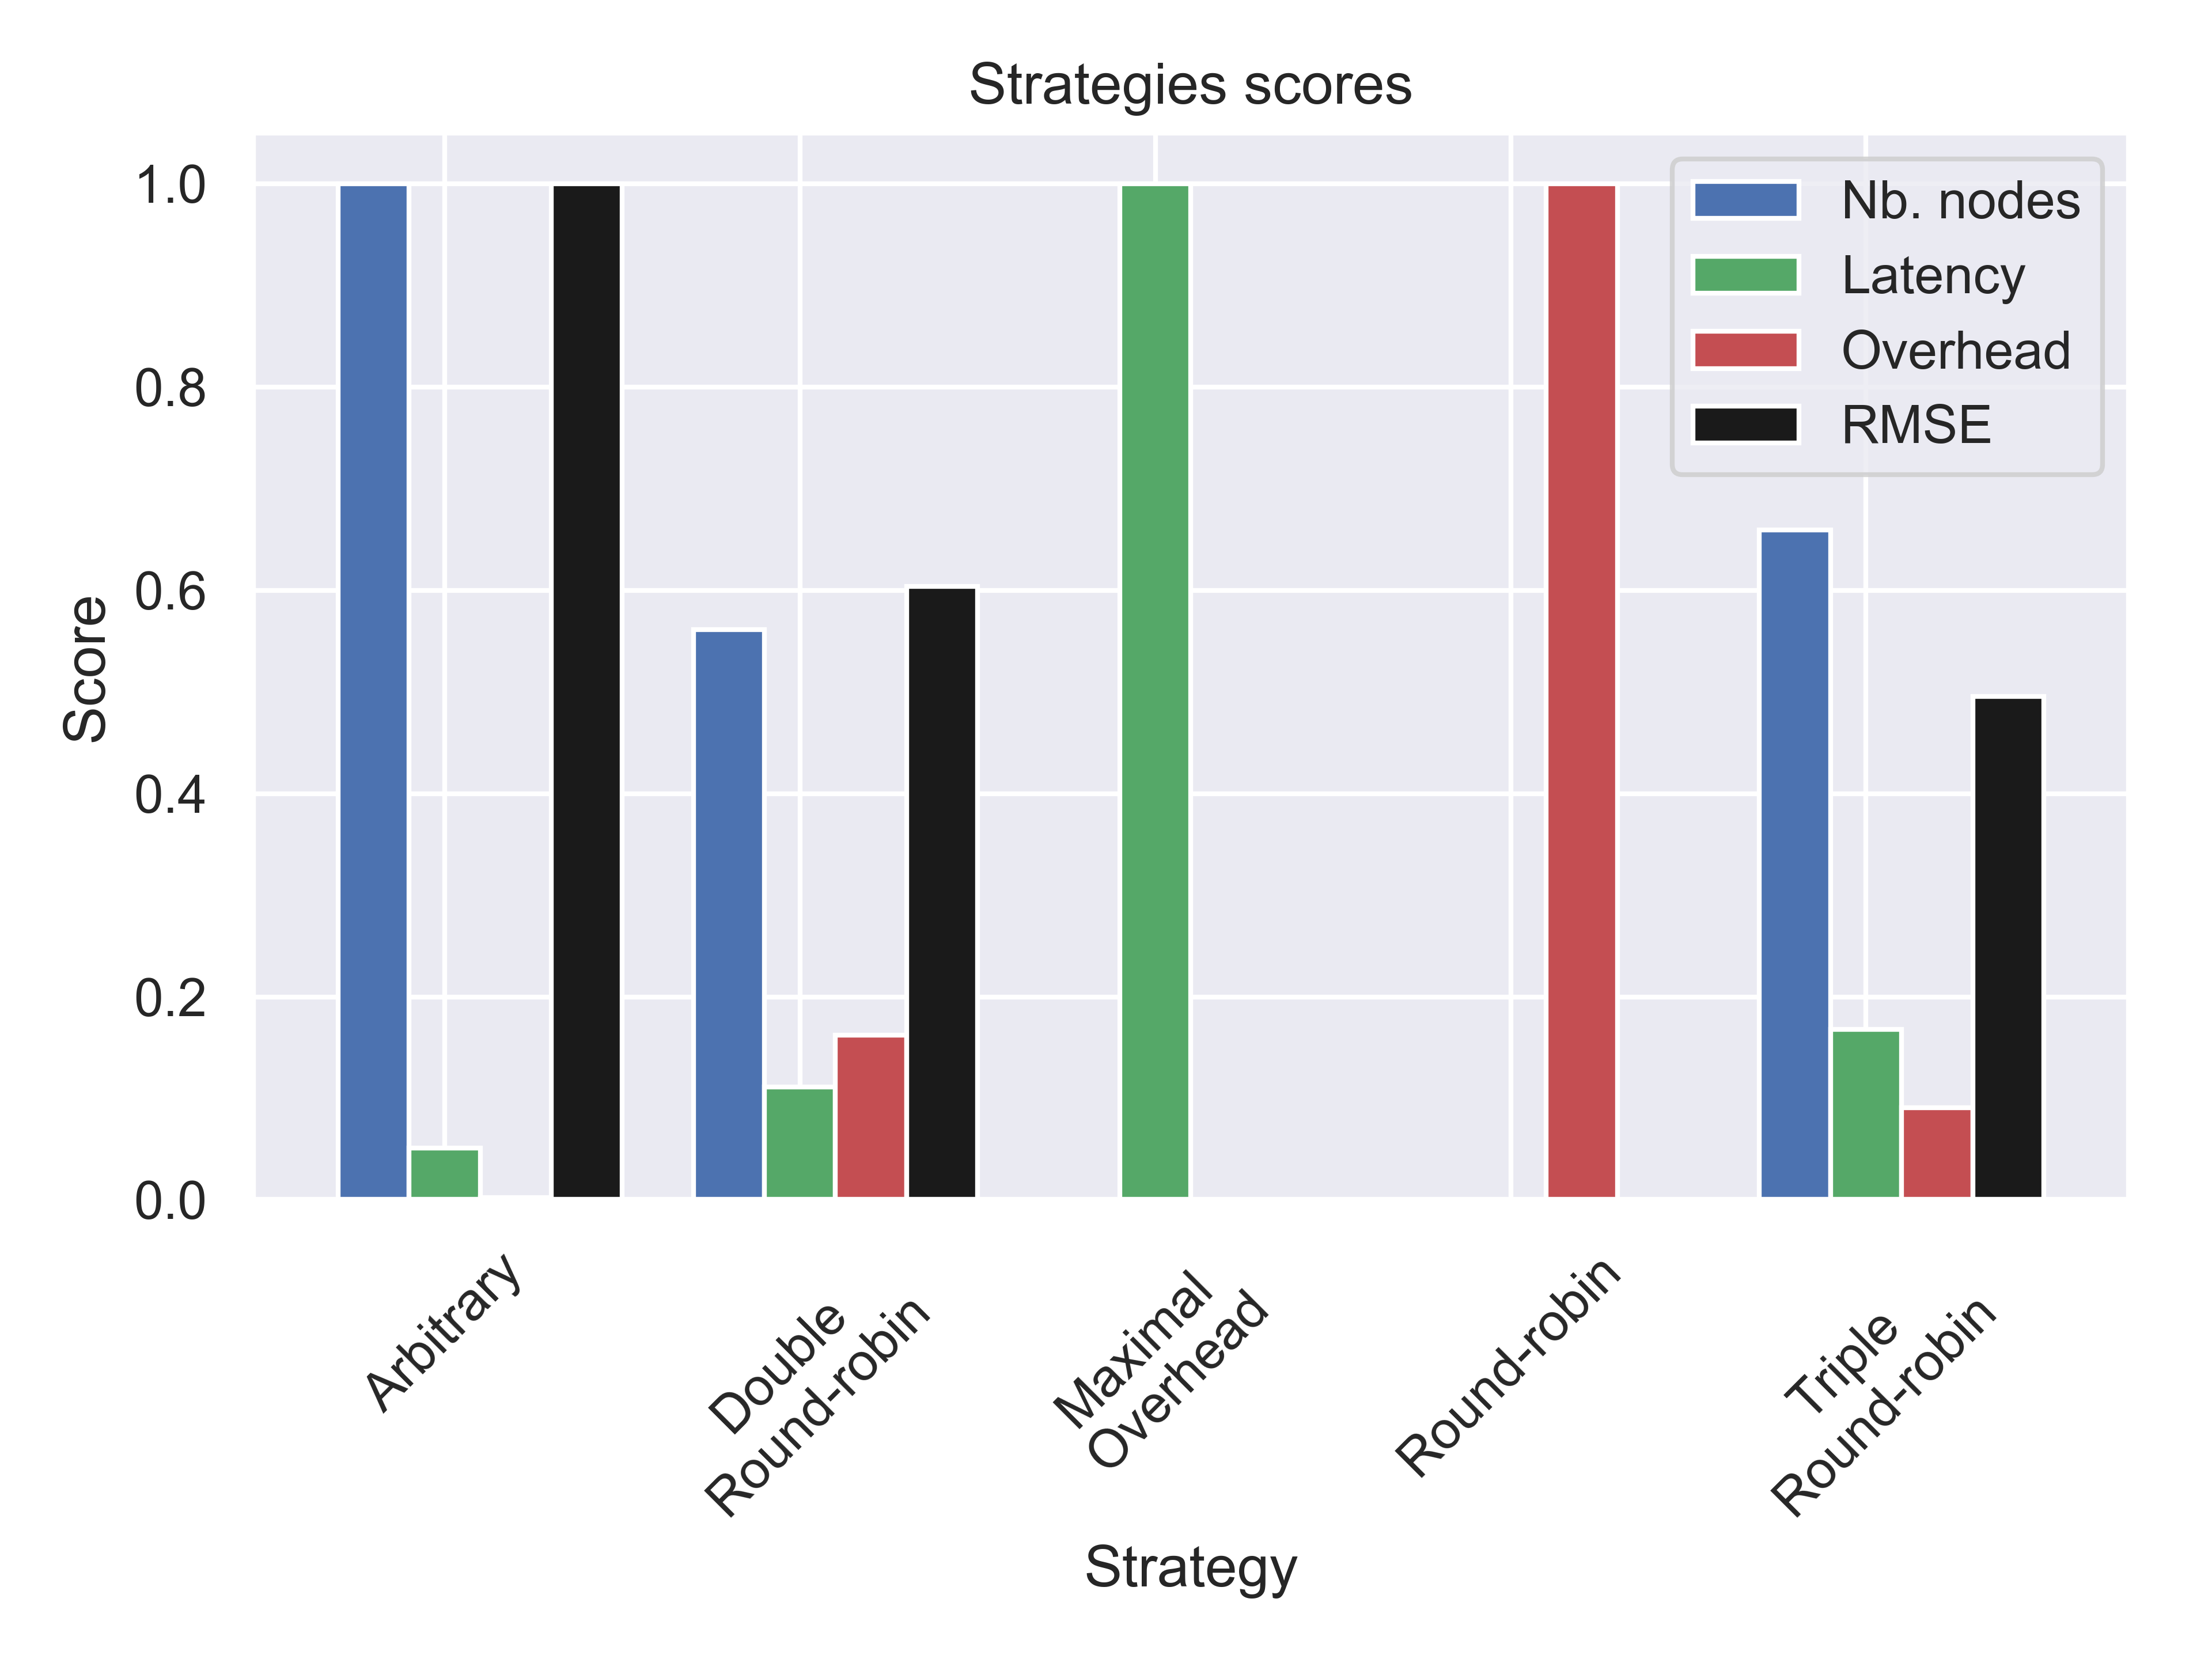
\includegraphics[width=0.8\columnwidth]{final_plot_norm_model}
    %\captionsetup{justification=centering}
    \caption{Normalized fitted values for the simple model. The strategies are listed
    on the x-axis and their scores are plotted along the y-axis. 
    This per-class normalization facilitates the comparison of strategies on one
    particular score.
    The correlation between the error score and the score for the number of
    nodes is also clearer when presented this way than, compared to the raw
    values.
    }
    \label{fig:recapTestsPlotNorm}
\end{figure}

\FloatBarrier
\subsection{Improvements of the basic model and new fitting}
\label{ssec:fittingImproved}
Now that there are exploitable results for the basic model, some improvements
can be made. The first step is to standardize the scale by imposing the range
\([0,1]\) which simplifies the visual juxtapisition as seen in
\fig{fig:recapTestsPlotNorm}. The next step is to try to give a meaning to
relative values for the same score when comparing two strategies. This is
obtained by finding better exponents for the variables in the model.

\subsubsection{Improving factors}
As seen in \ssec{ssec:fittingBase}, the best score for
the latency is \(0.5\), which is due to the fact that latency is at least \(2\).
A \(0.5\) factor can therefore be added to the model to obtain a value of \(1\)
as the maximum score for the latency:
\[1 = s_n \cdot \frac{1}{n} + \frac{1}{2} s_l\cdot l + s_o\cdot o\]
In the same manner, to scale the possible scores for the number of nodes to the
chosen interval of \([0,1]\), a factor of 2.556 can be added to the model:
\[1 = 2.556\cdot s_n \cdot \frac{1}{n} + \frac{1}{2} s_l\cdot l + s_o\cdot o\]
Both models are represented on \fig{fig:improvedFactors}

\doublefigure
    {final_plot_new_model_factor_latency}
    {final_plot_new_model_factor_latency_and_nodes}
    {Improvement of the factors of the basic model. On the left, the latency
    score has a maximum of \(1.0\). On the right, the score for the number of nodes
    is also normalized to a maximum of \(1.0\).
    }
    {fig:improvedFactors}


\subsubsection{Improving exponents}
Now that the model gives a normalized output, it is possible to improve it by
changing the exponents applied to the variables which could produce scores that
are easier to reason about. For example, as described in \ssec{ssec:doubleRR}
and \ssec{ssec:tripleRR} the
overhead for the double-round robin is 2/3 of the overhead for the triple
round-robin and, therefore, its score should be 3/2 of the overhead score for the
triple round-robin. 
However it seems it isn't the case as the score values in \tab{fig:recapTests}
for the double an triple round-robins are worth $0.162$ and $0.091$ and their
ratio amounts to $1.780$ but by performing a bisection on the function
\(\frac{0.162}{0.091}^e\) with a goal value of $3/2$, an exponent of
\(\frac{1}{2}\) is revealed.
As in \fig{fig:recapTestsPlotNew} and \tab{fig:recapTestsNew},using this newly
calculated exponent gives a much better ratio to the overhead score for each
round-robin strategy pair: single-double($2.092$), double-triple ($1.598$), and
single-triple ($3.344$).
Indeed, the overhead score for the single round-robin strategy
should be twice that of the double round robin strategy and three times as
much as the score for the triple round-robin. By looking at the error values
obtained by the fitting of the new model on the data
(\fig{fig:errorComparison}), it can be seen that those are marginally lower than
the original basic model, which means the model better fits the data that output
predictable results. 

The exponent for the latency is not to be changed because the scores already
match the expectations (the score for the triple round-robin is 3/2 of the score
for the double round-robin strategy). 

Again, the exponent for the number of nodes will not be modified because its
score's role in the model is to buffer.

The final model is therefore: 
\[1 = 2.556\cdot s_n \cdot \frac{1}{n} + \frac{1}{2} s_l\cdot l + s_o\cdot
\sqrt{o}\]

\begin{figure}[h]
    \centering
    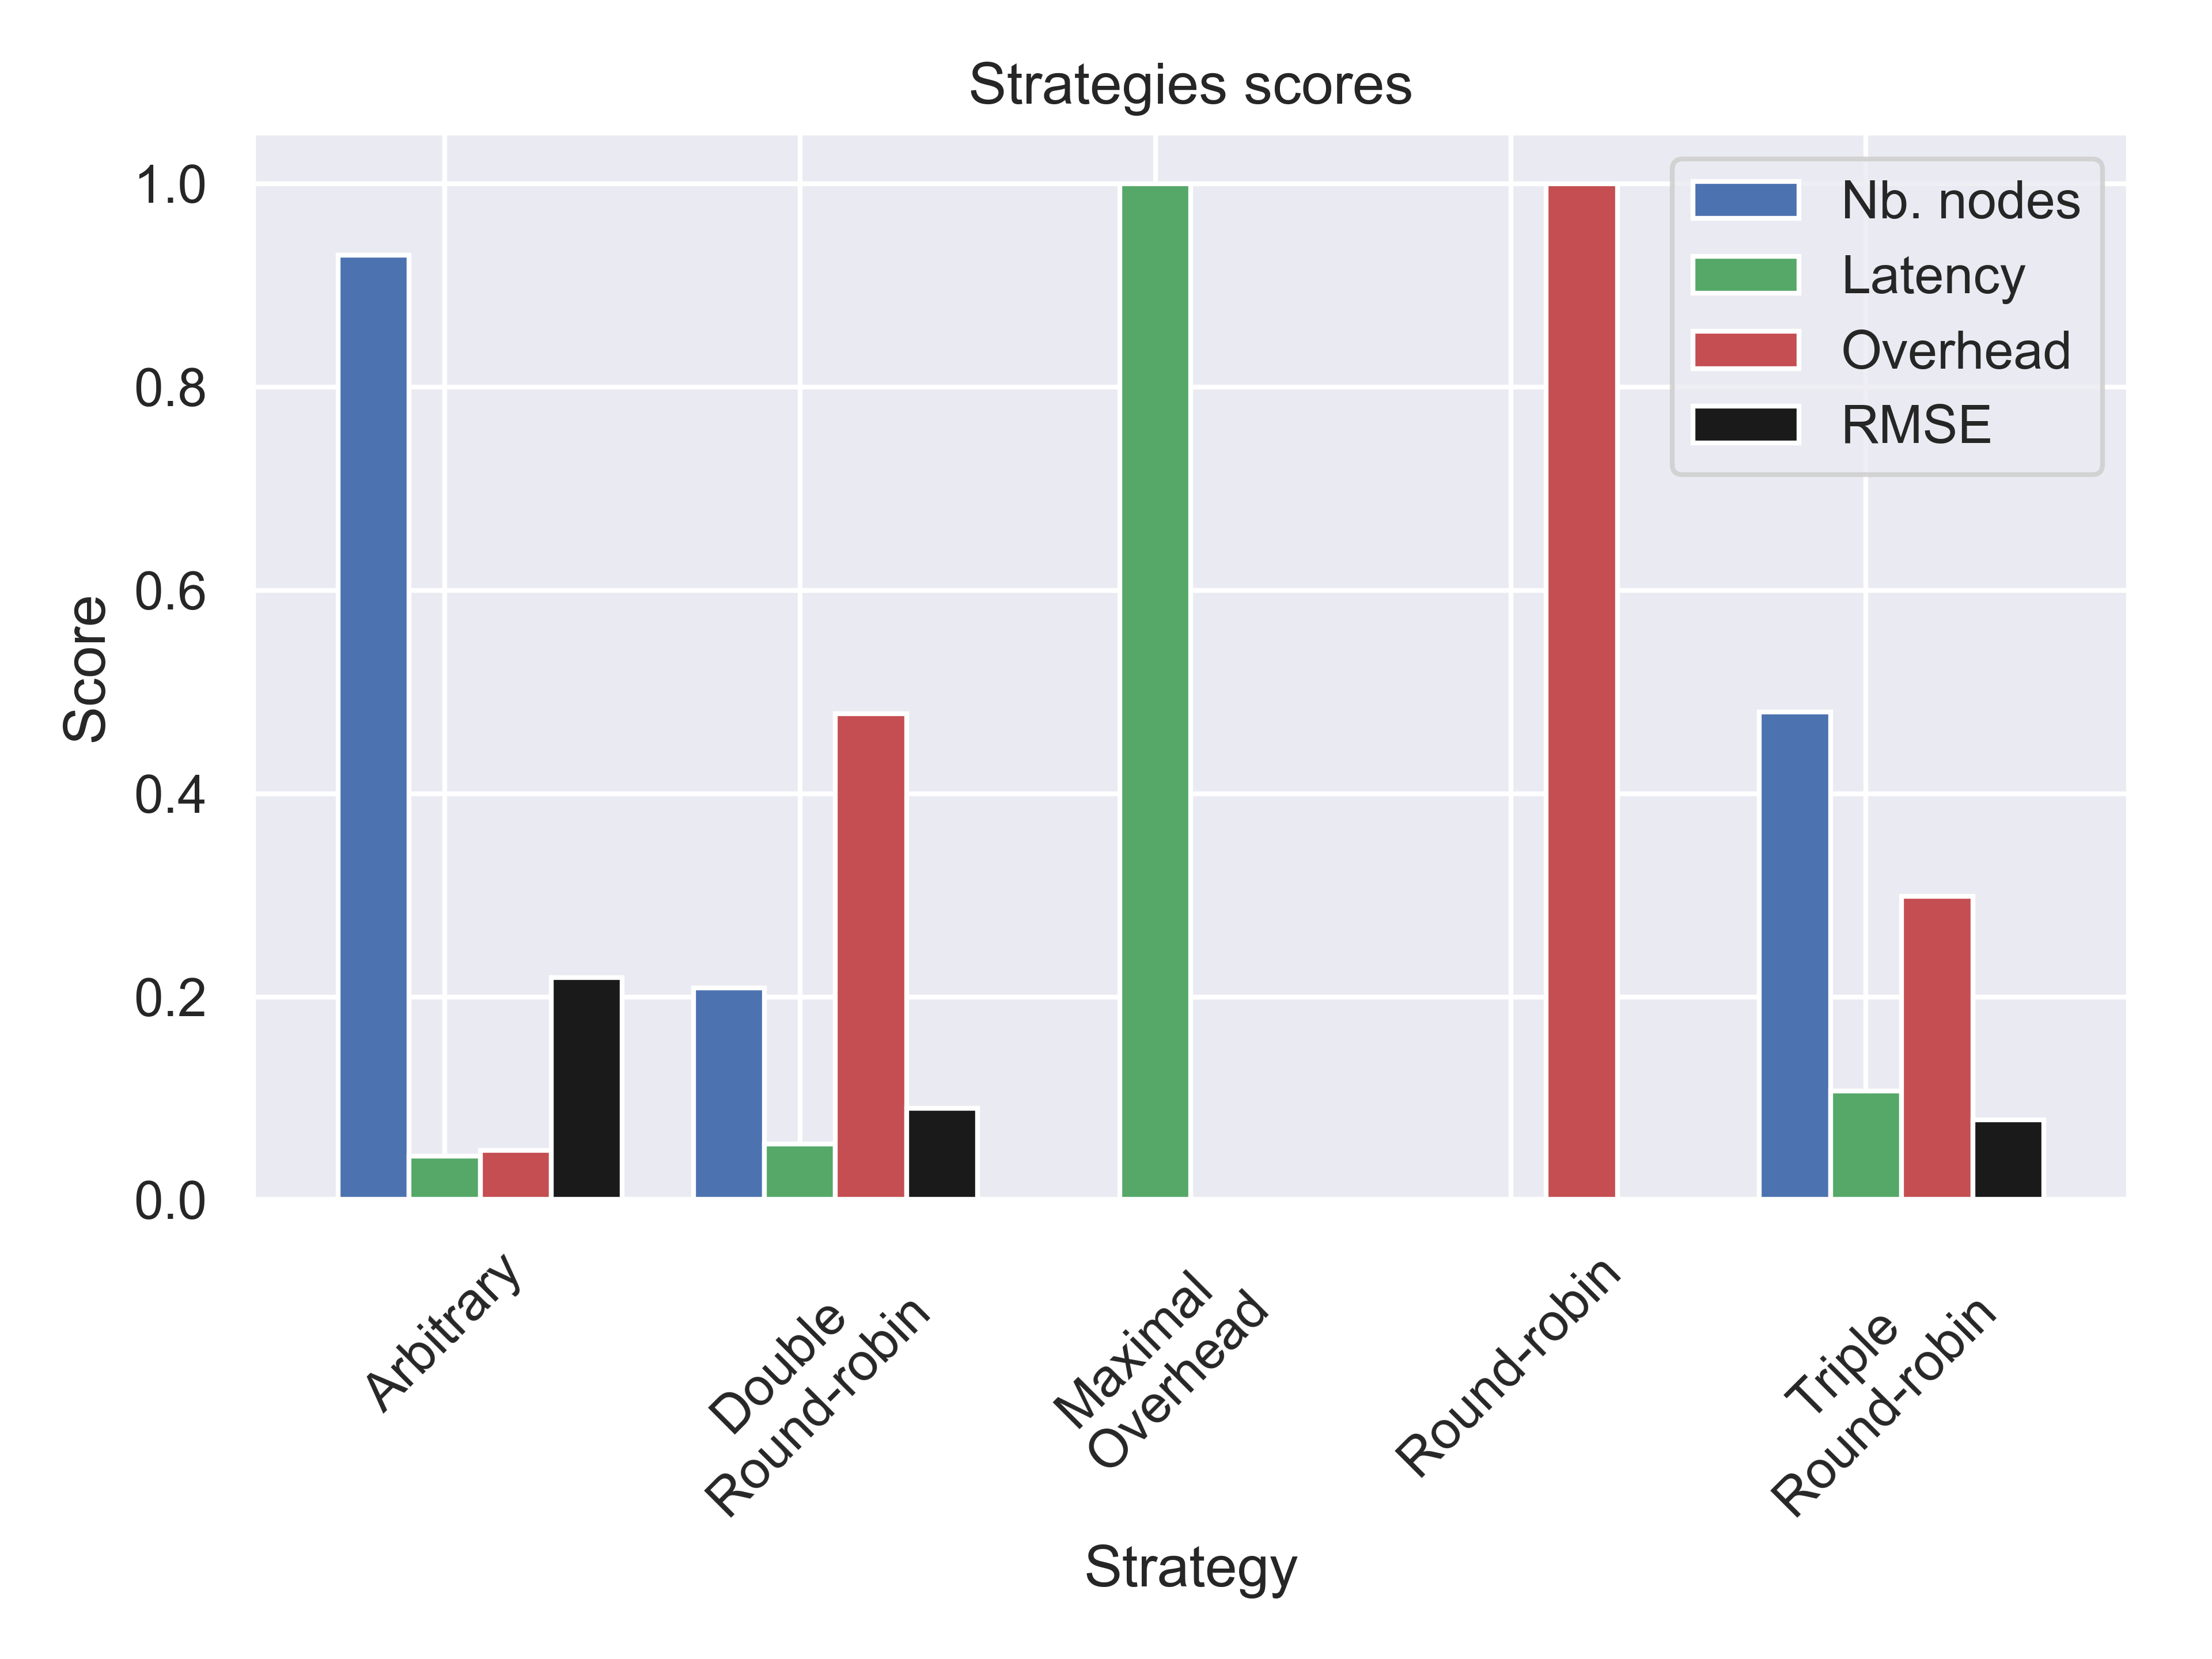
\includegraphics[width=0.8\columnwidth]{final_plot_new_model}
    %\captionsetup{justification=centering}
    \caption{Raw fitted values for the simple model, rounded to the 3rd
        decimal place. The RMSE column shows the error value for the linear
        regression. The scores are now normalized to the \([0, 1]\)
        interval. The new model also improves the relatives values for the
        overhead score, the double round-robin score is roughly half of
        the simple round-robin and the triple round-robin score is roughly a
        third of the overhead score for the simple round-robin strategy.}
    \label{fig:recapTestsPlotNew}
\end{figure}

\begin{table}[h]
    \centering{
        \begin{tabular}{|c|c|c|c|c|}
            \hline
            Sending Strategy & \(s_n\) & \(s_l\) & \(s_o\) & RMSE \\
            \hline
            Round-robin        & 0.000 & 0.000 & 1.000 & 0.000\\
            \hline
            Double round-robin & 0.209 & 0.055 & 0.478 & 0.090 \\
            \hline
            Triple round-robin & 0.480 & 0.107 & 0.299 & 0.079 \\
            \hline
            Maximal overhead   & 0.000 & 1.000 & 0.000 & 0.000 \\
            \hline
            \hline
            Arbitrary          & 0.929 & 0.043 & 0.049 & 0.219\\
            \hline
        \end{tabular}
       % %\captionsetup{justification=centering}
        \caption{Raw fitted values for the simple model, rounded to the 3rd
        decimal place. The RMSE column shows the error value for the linear
        regression. The scores are now normalized to the \([0, 1]\)
        interval. The new model also improves the relatives values for the
        overhead score, the double round-robin score is roughly half of 
        the simple round-robin and the triple round-robin score is roughly a
        third of the overhead score for the simple round-robin strategy.}
        \label{fig:recapTestsNew}
    }
\end{table}

\begin{table}[h]
    \centering{
        \begin{tabular}{|c|c|c|}
            \hline
            Sending Strategy & RMSE Basic model & RMSE Improved model \\
            \hline
            Round-robin        & 0.000 & 0.000\\
            \hline                     
            Double round-robin & 0.141 & 0.090 \\
            \hline                     
            Triple round-robin & 0.115 & 0.079 \\
            \hline                     
            Maximal overhead   & 0.000 & 0.000 \\
            \hline                     
            \hline                     
            Arbitrary          & 0.233 & 0.219\\
            \hline
        \end{tabular}
       % %\captionsetup{justification=centering}
        \caption{Raw error values for the simple and improved models, rounded to the 3rd
        decimal place. The error values are lower for the improved model which
        implies that it better fits the data.}
        \label{fig:errorComparison}
    }
\end{table}

\FloatBarrier
\section{Further research}
\subsection{Resolve edge case bug}
As discussed in \ssec{ssec:arbitrary}, an edge case bug has been identified at
the end of the project and it is necessary to fix this implementation error
before researching further on the subject.

\subsection{Half set strategy}
Another strategy that could be interesting to implement consists in 
half the validator set sends a message at each step. That would give a new
comparison point with a fixed latency and an overhead that would be half the one
for the Maximal overhead strategy. It would be useful to have it to find better
coefficients for the refined model.

\subsection{Bottom up strategies}
Now that the framework is functional and can give some reference points and has
ways to compare strategies, the next step would be to implement bottom
up strategies (see \ssec{ssec:bottomUpStrats}) that could include
rewarding/slashing the stake of the nodes.

\subsection{Optimize and simplify model}
As seen in Subsections \ref{ssec:fittingBase} and \ref{ssec:fittingImproved},
the model might be too restrictive for the actual problemi and it might be worth
trying to find a better fitting model to more precisely reproduce the real life
use case, by, for example, trying out new exponents for the number of nodes for
example. Removing the number of nodes as a whole in the model might also give
simpler data to analyse.

\subsection{Better network modeling}
Currently, the \texttt{proptest} implementation does not include a good model
for the network layer. The three proposed receiving strategies are naive but
allowed the validation of the framework from the metrics measurements to the actual
model fitting. A step forward would be to create better models for the
network, based on real life network topologies, latencies, number of nodes, etc.

\subsection{Further analyse the data}
As seen in \ssec{ssec:proptest}, more than one sending strategy have been
implemented, but only one has been thoroughly analysed. The some receivers
strategy was implemented early in the project for other purposes but it turned
out during the analysis phase that chosing both the number of nodes that receive
the message as well as which ones get them was too many varying parameters
added at once. The half receivers strategy was then implemented but data points
were generated too late into the project's lifetime to fully analyse them as
well. A logical next step would to use the half receivers strategy to validate
that the chosen model does not overfit the all receivers strategy data.
